\documentclass[fleqn]{article}
\usepackage[russian]{babel}
\usepackage{hyperref}
\usepackage[usenames,dvipsnames,svgnames,table,rgb]{xcolor}
\hypersetup{				% Гиперссылки
    unicode=true,           % русские буквы в раздела PDF
    colorlinks=true,       	% false: ссылки в рамках; true: цветные ссылки
    linkcolor=violet,          % внутренние ссылки
    citecolor=green,        % на библиографию
    filecolor=magenta,      % на файлы
    urlcolor=pink          % на URL
}

%% Created with wxMaxima 23.05.1

\setlength{\parskip}{\medskipamount}
\setlength{\parindent}{0pt}
\usepackage{iftex}
\ifPDFTeX
  % PDFLaTeX or LaTeX 
  \usepackage[utf8]{inputenc}
  \usepackage[T1]{fontenc}
  \DeclareUnicodeCharacter{00B5}{\ensuremath{\mu}}
\else
  %  XeLaTeX or LuaLaTeX
  \usepackage{fontspec}
\fi
\usepackage{graphicx}
\usepackage{color}
\usepackage{amsmath}
\usepackage{grffile}
\usepackage{ifthen}
\newsavebox{\picturebox}
\newlength{\pictureboxwidth}
\newlength{\pictureboxheight}
\newcommand{\includeimage}[1]{
    \savebox{\picturebox}{\includegraphics{#1}}
    \settoheight{\pictureboxheight}{\usebox{\picturebox}}
    \settowidth{\pictureboxwidth}{\usebox{\picturebox}}
    \ifthenelse{\lengthtest{\pictureboxwidth > .95\linewidth}}
    {
        \includegraphics[width=.75\linewidth,height=.60\textheight,keepaspectratio]{#1}
    }
    {
        \ifthenelse{\lengthtest{\pictureboxheight>.80\textheight}}
        {
            \includegraphics[width=.75\linewidth,height=.60\textheight,keepaspectratio]{#1}
            
        }
        {
            \includegraphics{#1}
        }
    }
}
\newlength{\thislabelwidth}
\DeclareMathOperator{\abs}{abs}

\definecolor{labelcolor}{RGB}{100,0,0}
\setlength{\topmargin}{-0.5in}
\setlength{\oddsidemargin}{0 in}
\textwidth 160mm
\textheight 220mm
\begin{document}

\thispagestyle{empty}
\begin{center}
% \singlespacing % Reset line spacing to 1 from here on
\setlength{\baselineskip}{8pt}

Министерство науки и высшего образования Российской Федерации

ФГАОУ ВО «Омский государственный университет им. Ф.М. Достоевского»

Факультет цифровых технологий и кибербезопасности

Кафедра компьютерной математики и программного обеспечения

Дисциплина: СиППО
\setlength{\baselineskip}{12pt}

\vspace*{15\baselineskip}
Лабораторная работа

"Задания по теории графов"

Вариант 2
\end{center}
\vspace*{10\baselineskip}
\begin{flushright}
    Выполнила:

Рузанова Д.П., ММБ-102-О-О2

Руководитель:

Агалаков С.А.
\end{flushright}
\vspace*{6\baselineskip}
\begin{center}
Омск 2024    
\end{center}
% \onehalfspacing
\newpage
\tableofcontents
\newpage
\section*{Задания по теории графов}
\addcontentsline{toc}{section}{Задания по теории графов}
\subsection*{Задание 1}
\addcontentsline{toc}{subsection}{Задание 1}
Загрузим специализированный пакет для работы с графами:\\

\noindent
%%%%%%%%
%% INPUT:
\begin{minipage}[t]{4.000000em}\color{red}\bfseries
(\% i1)	
\end{minipage}
\begin{minipage}[t]{\textwidth}\color{blue}
load(graphs)\$
\end{minipage}

\noindent%


Создадим неориентированный граф $G = (V,E)$ с множеством вершин $V$ и множеством ребер $E$.\\
$V=\{1,2,3,4,5,6\}$,\\
$E=\{  \{1,2\}, \{1,5\}, \{1,6\}, \{2,3\}, \{2,6\}, \{3,5\}, \{4,5\}, \{5,6\} \}$:\\
\noindent
%%%%%%%%
%% INPUT:
\begin{minipage}[t]{4.000000em}\color{red}\bfseries
(\% i2)	
\end{minipage}
\begin{minipage}[t]{\textwidth}\color{blue}
G:\ create\_graph([1,\ 2,\ 3,\ 4,\ 5,\ 6],\ [[1,\ 2],\ [1,\ 5],\ [1,\ 6],\ [2,\ 3],\ [2,\ 6],\ [3,5],\ [4,\ 5],\ [5,\ 6]]);
\end{minipage}
%%%% OUTPUT:
\[\displaystyle \tag{G} 
\ensuremath{\mathrm{GRAPH\backslash (6 vertices, 8 edges\backslash )}}\mbox{}
\]
%%%%%%%%%%%%%%%%


\noindent
%%%%%%%%
%% INPUT:
\begin{minipage}[t]{4.000000em}\color{red}\bfseries
(\% i3)	
\end{minipage}
\begin{minipage}[t]{\textwidth}\color{blue}
print\_graph(G);
\end{minipage}
%%%% OUTPUT:
\[\displaystyle Graph on 6 vertices with 8 edges.
Adjacencies:
  1 :  6  5  2
  2 :  6  3  1
  3 :  5  2
  4 :  5
  5 :  6  4  3  1
  6 :  5  2  1
\mbox{}\]


%%%%%%%%%%%%%%%%

\vspace*{1\baselineskip}
Построим изображение графа $G$ с помощью функции \textbf{$draw\_graph$}, используя опции, установленные по умолчанию:\\

\noindent
%%%%%%%%
%% INPUT:
\begin{minipage}[t]{4.000000em}\color{red}\bfseries
(\% i4)	
\end{minipage}
\begin{minipage}[t]{\textwidth}\color{blue}
draw\_graph(G);
\end{minipage}
%%%% OUTPUT:
\[\displaystyle \tag{\% t4} 
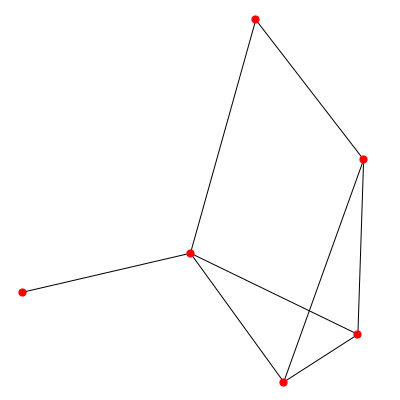
\includegraphics[width=.75\linewidth,height=.60\textheight,keepaspectratio]{graphs_img/graphs_1}\mbox{}\]


%%%%%%%%%%%%%%%%

Построим изображение графа $G$, на котором вершины графа помечены(метки слева от вершин), расположены в вершинах правильного многоугольника и окрашены в зеленый цвет:\\

\noindent
%%%%%%%%
%% INPUT:
\begin{minipage}[t]{4.000000em}\color{red}\bfseries
(\% i5)	
\end{minipage}
\begin{minipage}[t]{\textwidth}\color{blue}
draw\_graph(G,\ fixed\_vertices=[1,\ 2,\ 3,\ 4,\ 5,\ 6],\ show\_id=true,\ label\_alignment=right,\ \\
\ \ \ \ vertex\_color=green,\ redraw=true);
\end{minipage}
%%%% OUTPUT:
\[\displaystyle \tag{\% t5} 
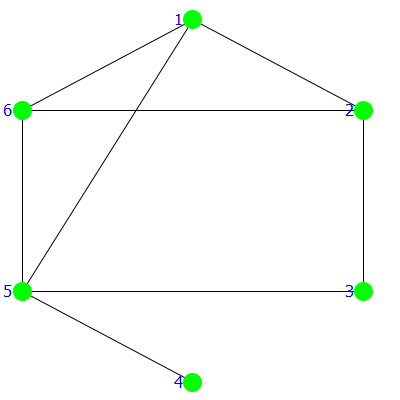
\includegraphics[width=.75\linewidth,height=.60\textheight,keepaspectratio]{graphs_img/graphs_2}\mbox{}\]


%%%%%%%%%%%%%%%%

Создадим дополнение $\overline{G}$ графа $G$:\\
\noindent
%%%%%%%%
%% INPUT:
\begin{minipage}[t]{4.000000em}\color{red}\bfseries
(\% i6)	
\end{minipage}
\begin{minipage}[t]{\textwidth}\color{blue}
G\_comp\ :\ complement\_graph(G);
\end{minipage}
%%%% OUTPUT:
\[\displaystyle \tag{G\_ comp} 
\ensuremath{\mathrm{GRAPH\backslash (6 vertices, 7 edges\backslash )}}\mbox{}
\]
%%%%%%%%%%%%%%%%

Построим изображение $\overline{G}$:\\
\noindent
%%%%%%%%
%% INPUT:
\begin{minipage}[t]{4.000000em}\color{red}\bfseries
(\% i7)	
\end{minipage}
\begin{minipage}[t]{\textwidth}\color{blue}
draw\_graph(G\_comp\ ,fixed\_vertices=[1,\ 2,\ 3,\ 4,\ 5,\ 6],\ show\_id=true,\ label\_alignment=right,\ \\
\ \ \ \ vertex\_color=green,\ redraw=true);
\end{minipage}
%%%% OUTPUT:
\[\displaystyle \tag{\% t7} 
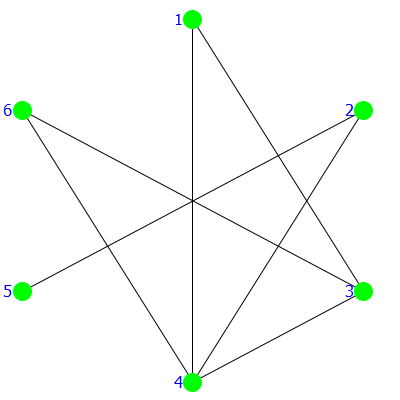
\includegraphics[width=.75\linewidth,height=.60\textheight,keepaspectratio]{graphs_img/graphs_3}\mbox{}\]

\[\tag{\% o7} 
\ensuremath{\mathrm{done}}\mbox{}
\]
%%%%%%%%%%%%%%%%

Найдем матрицу смежности графа $G$:\\
\noindent
%%%%%%%%
%% INPUT:
\begin{minipage}[t]{4.000000em}\color{red}\bfseries
(\% i8)	
\end{minipage}
\begin{minipage}[t]{\textwidth}\color{blue}
adjacency\_matrix(G);
\end{minipage}
%%%% OUTPUT:
\[\displaystyle \tag{\% o8} 
\begin{pmatrix}0 & 1 & 0 & 0 & 1 & 1\\
1 & 0 & 1 & 0 & 0 & 1\\
0 & 1 & 0 & 0 & 1 & 0\\
0 & 0 & 0 & 0 & 1 & 0\\
1 & 0 & 1 & 1 & 0 & 1\\
1 & 1 & 0 & 0 & 1 & 0\end{pmatrix}\mbox{}
\]
%%%%%%%%%%%%%%%%

Найдем матрицу смежности графа $\overline{G}$:\\
\noindent
%%%%%%%%
%% INPUT:
\begin{minipage}[t]{4.000000em}\color{red}\bfseries
(\% i9)	
\end{minipage}
\begin{minipage}[t]{\textwidth}\color{blue}
adjacency\_matrix(G\_comp);
\end{minipage}
%%%% OUTPUT:
\[\displaystyle \tag{\% o9} 
\begin{pmatrix}0 & 0 & 1 & 1 & 0 & 0\\
0 & 0 & 0 & 0 & 1 & 0\\
1 & 0 & 0 & 1 & 1 & 1\\
1 & 0 & 1 & 0 & 0 & 1\\
0 & 1 & 1 & 0 & 0 & 0\\
0 & 0 & 1 & 1 & 0 & 0\end{pmatrix}\mbox{}
\]
%%%%%%%%%%%%%%%%

Создадим копию графа $G$:\\
\noindent
%%%%%%%%
%% INPUT:
\begin{minipage}[t]{4.000000em}\color{red}\bfseries
(\% i10)	
\end{minipage}
\begin{minipage}[t]{\textwidth}\color{blue}
graph\_copy:\ copy\_graph(G);
\end{minipage}
%%%% OUTPUT:
\[\displaystyle \tag{graph\_ copy} 
\ensuremath{\mathrm{GRAPH\backslash (6 vertices, 8 edges\backslash )}}\mbox{}
\]
%%%%%%%%%%%%%%%%

\subsection*{Задание 2}
\addcontentsline{toc}{subsection}{Задание 2}

Создадим граф $G_1$ по его матрице смежности \\
\left[\begin{array}{cccccc}
    0 & 1 & 1 & 0 & 0 & 0\\
    1 & 0 & 1 & 0 & 1 & 1\\
    1 & 1 & 0 & 0 & 0 & 0\\
    0 & 0 & 0 & 0 & 1 & 0\\
    0 & 1 & 0 & 1 & 0 & 1\\
    0 & 1 & 0 & 0 & 1 & 0
\end{array}\right]$$

\noindent
%%%%%%%%
%% INPUT:
\begin{minipage}[t]{4.000000em}\color{red}\bfseries
(\% i11)	
\end{minipage}
\begin{minipage}[t]{\textwidth}\color{blue}
G1\ :\ from\_adjacency\_matrix(matrix(\\
\ \ \ \ \ \ \ \ [0,\ 1,\ 1,\ 0,\ 0,\ 0],\ \\
\ \ \ \ \ \ \ \ [1,\ 0,\ 1,\ 0,\ 1,\ 1],\ \\
\ \ \ \ \ \ \ \ [1,\ 1,\ 0,\ 0,\ 0,\ 0],\ \\
\ \ \ \ \ \ \ \ [0,0,0,0,1,\ 0],\\
\ \ \ \ \ \ \ \ [0,\ 1,\ 0,\ 1,\ 0,\ 1],\ \\
\ \ \ \ \ \ \ \ [0,\ 1\ ,\ 0,\ 0,\ 1,\ 0]));
\end{minipage}
%%%% OUTPUT:
\[\displaystyle \tag{G1} 
\ensuremath{\mathrm{GRAPH\backslash (6 vertices, 7 edges\backslash )}}\mbox{}
\]
%%%%%%%%%%%%%%%%

Построим изображение графа $G_1$, на котором помечены вершины графа(метки слева от вершин):\\

\noindent
%%%%%%%%
%% INPUT:
\begin{minipage}[t]{4.000000em}\color{red}\bfseries
(\% i12)	
\end{minipage}
\begin{minipage}[t]{\textwidth}\color{blue}
draw\_graph(G1,\ fixed\_vertices=[0,\ 1,\ 2,3,\ 4,5\ ],show\_id=true,\ label\_alignment=right,\ redraw=true);
\end{minipage}
%%%% OUTPUT:
\[\displaystyle \tag{\% t12} 
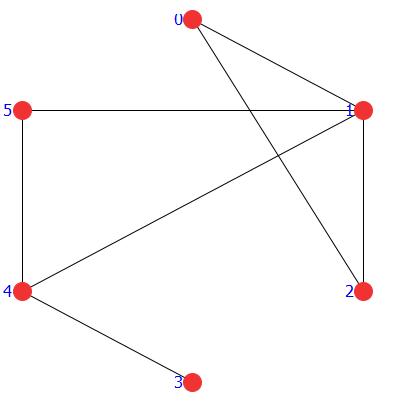
\includegraphics[width=.75\linewidth,height=.60\textheight,keepaspectratio]{graphs_img/graphs_4}\mbox{}\]

\[\tag{\% o12} 
\ensuremath{\mathrm{done}}\mbox{}
\]
%%%%%%%%%%%%%%%%

\subsection*{Задание 3}
\addcontentsline{toc}{subsection}{Задание 3}
Создадим орграф $G_2$ с множеством вершин $V$ и множеством дуг $E$.\\
$V=\{1,2,3,4,5,6\}$,\\
$E=\{  \{1,2\}, \{2,4\}, \{2,5\}, \{2,6\}, \{3,5\}, \{3,6\}, \{4,6\}, \{5,2\} ,\{5,4\},\{6,1\}\}$:\\

\noindent
%%%%%%%%
%% INPUT:
\begin{minipage}[t]{4.000000em}\color{red}\bfseries
(\% i13)	
\end{minipage}
\begin{minipage}[t]{\textwidth}\color{blue}
\ G\_2:\ create\_graph([1,\ 2,\ 3,\ 4,\ 5,\ 6],\ [[1,\ 2],\ [2,4],\ [2,\ 5],\ [2,\ 6],\ [3,5],\ [3,6],\ [4,\ 6],\ [5,\ 2],\ [5,\ 4],\ [6,\ 1]],\ directed=true);
\end{minipage}
%%%% OUTPUT:
\[\displaystyle \tag{G\_ 2} 
\ensuremath{\mathrm{DIGRAPH\backslash (6 vertices, 10 arcs\backslash )}}\mbox{}
\]
%%%%%%%%%%%%%%%%

Построим изображение орграфа $G_2$ на котором вершины помечены(метки по центру), расположены в вершинах правильного многоугольника, а дуги раскрашены в синий цвет:\\
\noindent
%%%%%%%%
%% INPUT:
\begin{minipage}[t]{4.000000em}\color{red}\bfseries
(\% i14)	
\end{minipage}
\begin{minipage}[t]{\textwidth}\color{blue}
draw\_graph(G\_2,fixed\_vertices=[1,\ 2,\ 3,\ 4,\ 5,\ 6],\ show\_id=true,\ edge\_color=blue,\ label\_alignment=center);
\end{minipage}
%%%% OUTPUT:
\[\displaystyle \tag{\% t14} 
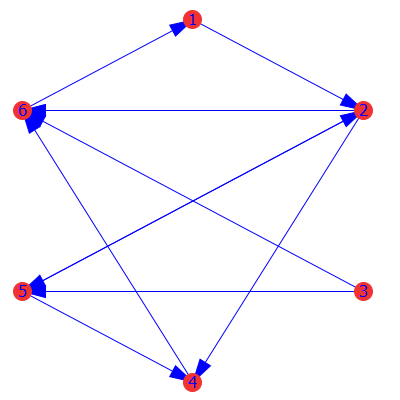
\includegraphics[width=.75\linewidth,height=.60\textheight,keepaspectratio]{graphs_img/graphs_5}\mbox{}\]


%%%%%%%%%%%%%%%%

Найдем матрицу смежности орграфа $G_2$:\\
\noindent
%%%%%%%%
%% INPUT:
\begin{minipage}[t]{4.000000em}\color{red}\bfseries
(\% i15)	
\end{minipage}
\begin{minipage}[t]{\textwidth}\color{blue}
adjacency\_matrix(G\_2);
\end{minipage}
%%%% OUTPUT:
\[\displaystyle \tag{\% o15} 
\begin{pmatrix}0 & 0 & 0 & 0 & 0 & 1\\
1 & 0 & 0 & 0 & 1 & 0\\
0 & 0 & 0 & 0 & 0 & 0\\
0 & 1 & 0 & 0 & 1 & 0\\
0 & 1 & 1 & 0 & 0 & 0\\
0 & 1 & 1 & 1 & 0 & 0\end{pmatrix}\mbox{}
\]
%%%%%%%%%%%%%%%%

\subsection*{Задание 4}
\addcontentsline{toc}{subsection}{Задание 4}
Создадим пустой 9-вершинный граф $O_9$ и построим его изображение:\\
\noindent
%%%%%%%%
%% INPUT:
\begin{minipage}[t]{4.000000em}\color{red}\bfseries
(\% i17)	
\end{minipage}
\begin{minipage}[t]{\textwidth}\color{blue}
O\_9\ :\ empty\_graph(9);\\
draw\_graph(O\_9,\ fixed\_vertices=[0,\ 1,\ 2,\ 3,\ 4,\ 5,\ 6,\ 7,\ 8\ ]);
\end{minipage}
%%%% OUTPUT:
\[\displaystyle \tag{O\_ 9} 
\ensuremath{\mathrm{GRAPH\backslash (9 vertices, 0 edges\backslash )
}}\mbox{}\]

\[\tag{\% t17} 
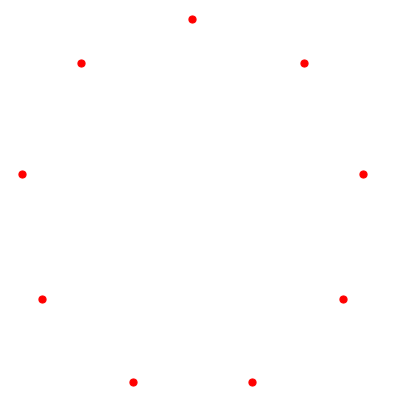
\includegraphics[width=.75\linewidth,height=.60\textheight,keepaspectratio]{graphs_img/graphs_6}\mbox{}\]


%%%%%%%%%%%%%%%%



Создадим полный 6-вершинный граф $K_{6}$ и построим его изображение:\\
\noindent
%%%%%%%%
%% INPUT:
\begin{minipage}[t]{4.000000em}\color{red}\bfseries
(\% i19)	
\end{minipage}
\begin{minipage}[t]{\textwidth}\color{blue}
K\_6\ :\ complete\_graph(6);\\
draw\_graph(K\_6);
\end{minipage}
%%%% OUTPUT:
\[\displaystyle \tag{K\_ 6} 
\ensuremath{\mathrm{GRAPH\backslash (6 vertices, 15 edges\backslash )
}}\mbox{}\]

\[\tag{\% t19} 
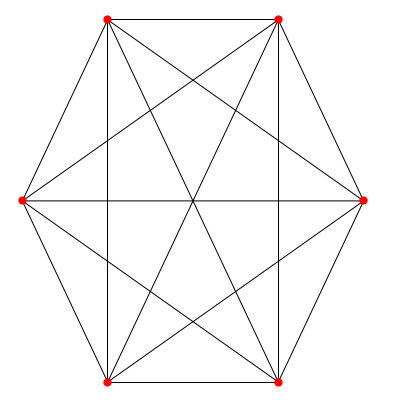
\includegraphics[width=.75\linewidth,height=.60\textheight,keepaspectratio]{graphs_img/graphs_7}\mbox{}\]


%%%%%%%%%%%%%%%%


Создадим полный двудольный граф $K_{3,5}$ и построим его изображение:\\
\noindent
%%%%%%%%
%% INPUT:
\begin{minipage}[t]{4.000000em}\color{red}\bfseries
(\% i21)	
\end{minipage}
\begin{minipage}[t]{\textwidth}\color{blue}
K\ :\ complete\_bipartite\_graph(3,\ 5);\\
draw\_graph(K,\ show\_id=true);
\end{minipage}
%%%% OUTPUT:
\[\displaystyle \tag{K} 
\ensuremath{\mathrm{GRAPH\backslash (8 vertices, 15 edges\backslash )
}}\mbox{}\]

\[\tag{\% t21} 
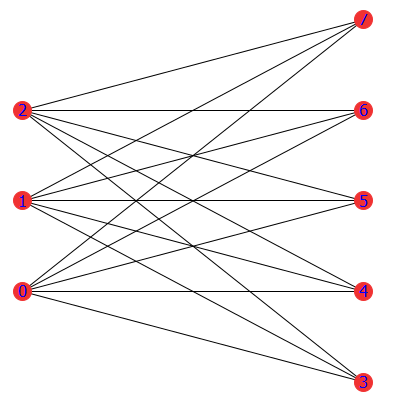
\includegraphics[width=.75\linewidth,height=.60\textheight,keepaspectratio]{graphs_img/graphs_8}\mbox{}\]

\[\tag{\% o21} 
\ensuremath{\mathrm{done}}\mbox{}
\]
%%%%%%%%%%%%%%%%

Создадим простую цепь $P_{6}$ и построим её изображение:\\

\noindent
%%%%%%%%
%% INPUT:
\begin{minipage}[t]{4.000000em}\color{red}\bfseries
(\% i23)	
\end{minipage}
\begin{minipage}[t]{\textwidth}\color{blue}
P\_6:\ path\_graph(6);\\
draw\_graph(P\_6);
\end{minipage}
%%%% OUTPUT:
\[\displaystyle \tag{P\_ 6} 
\ensuremath{\mathrm{GRAPH\backslash (6 vertices, 5 edges\backslash )
}}\mbox{}\]

\[\tag{\% t23} 
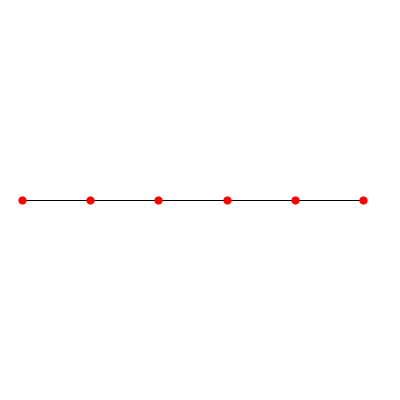
\includegraphics[width=.75\linewidth,height=.60\textheight,keepaspectratio]{graphs_img/graphs_9}\mbox{}\]


%%%%%%%%%%%%%%%%

Создадим простой 5-вершинный цикл $C_{9}$ и построим его изображение:\\
\noindent
%%%%%%%%
%% INPUT:
\begin{minipage}[t]{4.000000em}\color{red}\bfseries
(\% i25)	
\end{minipage}
\begin{minipage}[t]{\textwidth}\color{blue}
C\_9:\ cycle\_graph(9);\\
draw\_graph(C\_9);
\end{minipage}
%%%% OUTPUT:
\[\displaystyle \tag{C\_ 9} 
\ensuremath{\mathrm{GRAPH\backslash (9 vertices, 9 edges\backslash )
}}\mbox{}\]

\[\tag{\% t25} 
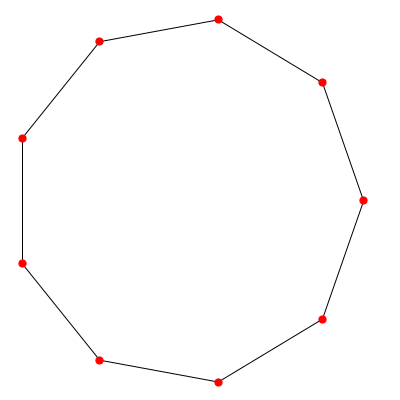
\includegraphics[width=.75\linewidth,height=.60\textheight,keepaspectratio]{graphs_img/graphs_10}\mbox{}\]

\[\tag{\% o25} 
\ensuremath{\mathrm{done}}\mbox{}
\]
%%%%%%%%%%%%%%%%

Создадим граф куба $Q_{4}$ и построим его изображение:\\
\noindent
%%%%%%%%
%% INPUT:
\begin{minipage}[t]{4.000000em}\color{red}\bfseries
(\% i27)	
\end{minipage}
\begin{minipage}[t]{\textwidth}\color{blue}
Q\_4:\ cube\_graph(4);\\
draw\_graph(Q\_4);
\end{minipage}
%%%% OUTPUT:
\[\displaystyle \tag{Q\_ 4} 
\ensuremath{\mathrm{GRAPH\backslash (16 vertices, 32 edges\backslash )
}}\mbox{}\]

\[\tag{\% t27} 
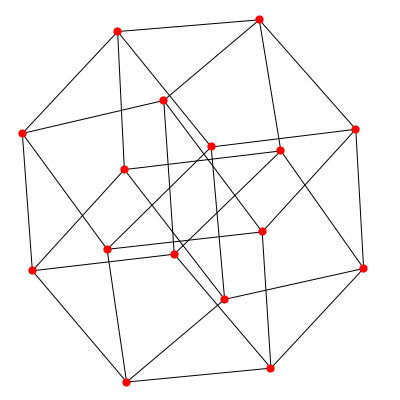
\includegraphics[width=.75\linewidth,height=.60\textheight,keepaspectratio]{graphs_img/graphs_11}\mbox{}\]


%%%%%%%%%%%%%%%%

Создадим граф колеса $W_9$ и построим его изображение:\\
\noindent
%%%%%%%%
%% INPUT:
\begin{minipage}[t]{4.000000em}\color{red}\bfseries
(\% i29)	
\end{minipage}
\begin{minipage}[t]{\textwidth}\color{blue}
W\_9\ :\ wheel\_graph(9);\\
draw\_graph(W\_9);
\end{minipage}
%%%% OUTPUT:
\[\displaystyle \tag{W\_ 9} 
\ensuremath{\mathrm{GRAPH\backslash (10 vertices, 18 edges\backslash )
}}\mbox{}\]

\[\tag{\% t29} 
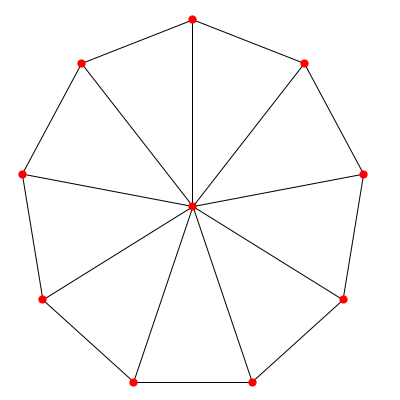
\includegraphics[width=.75\linewidth,height=.60\textheight,keepaspectratio]{graphs_img/graphs_12}\mbox{}\]


%%%%%%%%%%%%%%%%

Создадим граф Петерсена и построим его изображение:\\
\noindent
%%%%%%%%
%% INPUT:
\begin{minipage}[t]{4.000000em}\color{red}\bfseries
(\% i31)	
\end{minipage}
\begin{minipage}[t]{\textwidth}\color{blue}
petersen:\ petersen\_graph();\\
draw\_graph(petersen);
\end{minipage}
%%%% OUTPUT:
\[\displaystyle \tag{petersen} 
\ensuremath{\mathrm{GRAPH\backslash (10 vertices, 15 edges\backslash )
}}\mbox{}\]

\[\tag{\% t31} 
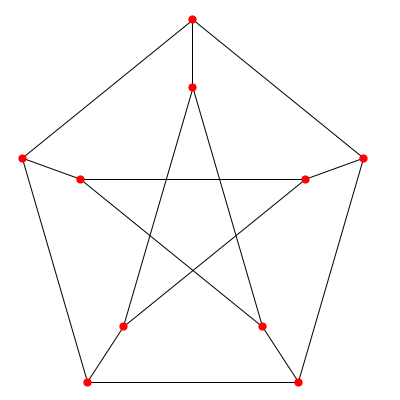
\includegraphics[width=.75\linewidth,height=.60\textheight,keepaspectratio]{graphs_img/graphs_13}\mbox{}\]

%%%%%%%%%%%%%%%%

\subsection*{Задание 5}
\addcontentsline{toc}{subsection}{Задание 5}
Создадим случайный граф с 6 вершинами, каждое ребро которого присутствует с вероятностью 0,7 и построим его изображение, предварительно пометив вершины:\\
\noindent
%%%%%%%%
%% INPUT:
\begin{minipage}[t]{4.000000em}\color{red}\bfseries
(\% i33)	
\end{minipage}
\begin{minipage}[t]{\textwidth}\color{blue}
R:\ random\_graph(6,\ 0.7);\\
draw\_graph(R,\ fixed\_vertices=[0,\ 1,\ 2,3,\ 4,5\ ],show\_id=true,\ label\_alignment=right,\ redraw=true);
\end{minipage}
%%%% OUTPUT:
\[\displaystyle \tag{R} 
\ensuremath{\mathrm{GRAPH\backslash (6 vertices, 12 edges\backslash )
}}\mbox{}\]

\[\tag{\% t33} 
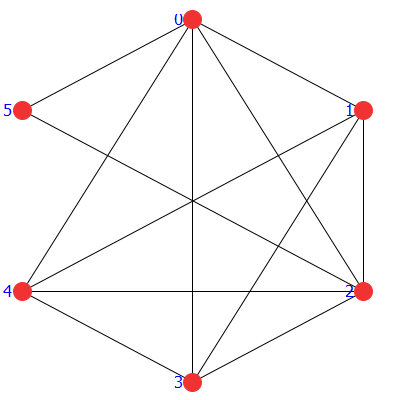
\includegraphics[width=.75\linewidth,height=.60\textheight,keepaspectratio]{graphs_img/graphs_14}\mbox{}\]

%%%%%%%%%%%%%%%%

Создадим случайный орграф с 8 вершинами, каждое ребро которого присутствует с вероятностью 0,3 и построим его изображение, предварительно пометив вершины:\\
\noindent
%%%%%%%%
%% INPUT:
\begin{minipage}[t]{4.000000em}\color{red}\bfseries
(\% i35)	
\end{minipage}
\begin{minipage}[t]{\textwidth}\color{blue}
R1:\ random\_digraph(8,\ 0.3);\\
draw\_graph(R1,\ fixed\_vertices=[0,\ 1,\ 2,3,\ 4,5\ ,\ 6,\ 7],show\_id=true,\ redraw=true);
\end{minipage}
%%%% OUTPUT:
\[\displaystyle \tag{R1} 
\ensuremath{\mathrm{DIGRAPH\backslash (8 vertices, 19 arcs\backslash )
}}\mbox{}\]

\[\tag{\% t35} 
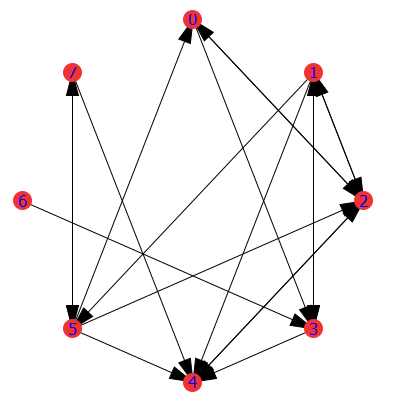
\includegraphics[width=.75\linewidth,height=.60\textheight,keepaspectratio]{graphs_img/graphs_15}\mbox{}\]

\[\tag{\% o35} 
\ensuremath{\mathrm{done}}\mbox{}
\]
%%%%%%%%%%%%%%%%

\subsection*{Задание 6}
\addcontentsline{toc}{subsection}{Задание 6}
Создадим случайный двудольный граф с числом вершин $5+7$, каждое ребро которого присутствуют с вероятностью с вероятностью 0,6. Визуализируем номера вершин графа(метки по центру). Разобьем множество вершин графа на доли и построим его изображение, на котором вершины, принадлежащие разным долям, окрашены в разные цвета:\\
\noindent
%%%%%%%%
%% INPUT:
\begin{minipage}[t]{4.000000em}\color{red}\bfseries
(\% i38)	
\end{minipage}
\begin{minipage}[t]{\textwidth}\color{blue}
R2:\ random\_bipartite\_graph(5,\ 7,\ 0.6);\\
[A,\ B]:\ bipartition(R2);\\
draw\_graph(R2,\ fixed\_vertices=makelist(i,i,0,13,1),show\_id=true,show\_vertices=A,\ redraw=true);
\end{minipage}
%%%% OUTPUT:
\[\displaystyle \tag{R2} 
\ensuremath{\mathrm{GRAPH\backslash (12 vertices, 19 edges\backslash )
}}\mbox{}\]

\[\tag{\% o37} 
\left[ \left[ 1\operatorname{,}4\operatorname{,}2\operatorname{,}0\operatorname{,}3\right] \operatorname{,}\left[ 11\operatorname{,}9\operatorname{,}7\operatorname{,}10\operatorname{,}8\operatorname{,}5\operatorname{,}6\right] \right] \mbox{}\]

\[\tag{\% t38} 
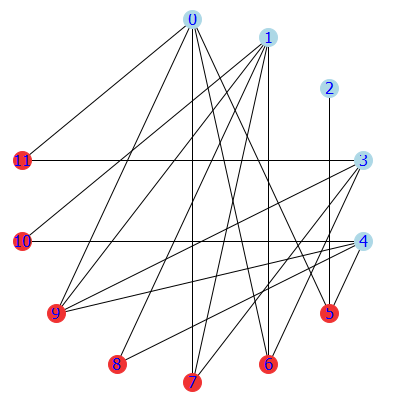
\includegraphics[width=.75\linewidth,height=.60\textheight,keepaspectratio]{graphs_img/graphs_16}\mbox{}\]

\[\tag{\% o38} 
\ensuremath{\mathrm{done}}\mbox{}
\]
%%%%%%%%%%%%%%%%

\subsection*{Задание 7}
\addcontentsline{toc}{subsection}{Задание 7}
Создадим случайный граф F с 20 вершинами и 100 ребрами.\\
Для наглядности построим его изображение.\\
Выясним, является ли созданный граф связным, деревом, двудольным, гамильтоновым, планарным:\\
\noindent
%%%%%%%%
%% INPUT:
\begin{minipage}[t]{4.000000em}\color{red}\bfseries
(\% i40)	
\end{minipage}
\begin{minipage}[t]{\textwidth}\color{blue}
F:\ random\_graph1(20,\ 100);\\
draw\_graph(F,\ fixed\_vertices=makelist(i,i,0,19,1),show\_id=true,\ vertex\_color=light\_blue,\ redraw=true);\\

\end{minipage}
%%%% OUTPUT:
\[\displaystyle \tag{F} 
\ensuremath{\mathrm{GRAPH\backslash (20 vertices, 100 edges\backslash )
}}\mbox{}\]

\[\tag{\% t40} 
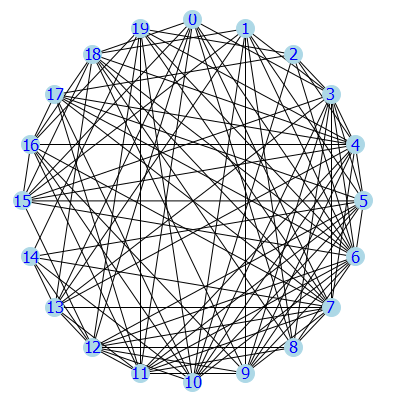
\includegraphics[width=.75\linewidth,height=.60\textheight,keepaspectratio]{graphs_img/graphs_17}\mbox{}\]


%%%%%%%%%%%%%%%%


\noindent
%%%%%%%%
%% INPUT:
\begin{minipage}[t]{4.000000em}\color{red}\bfseries
(\% i41)	
\end{minipage}
\begin{minipage}[t]{\textwidth}\color{blue}
is\_connected(F);
\end{minipage}
%%%% OUTPUT:
\[\displaystyle \tag{\% o41} 
true\mbox{}
\]
%%%%%%%%%%%%%%%%


\noindent
%%%%%%%%
%% INPUT:
\begin{minipage}[t]{4.000000em}\color{red}\bfseries
(\% i42)	
\end{minipage}
\begin{minipage}[t]{\textwidth}\color{blue}
is\_tree(F);
\end{minipage}
%%%% OUTPUT:
\[\displaystyle \tag{\% o42} 
false\mbox{}
\]
%%%%%%%%%%%%%%%%


\noindent
%%%%%%%%
%% INPUT:
\begin{minipage}[t]{4.000000em}\color{red}\bfseries
(\% i43)	
\end{minipage}
\begin{minipage}[t]{\textwidth}\color{blue}
is\_bipartite(F);\\

\end{minipage}
%%%% OUTPUT:
\[\displaystyle \tag{\% o43} 
false\mbox{}
\]
%%%%%%%%%%%%%%%%


\noindent
%%%%%%%%
%% INPUT:
\begin{minipage}[t]{4.000000em}\color{red}\bfseries
(\% i44)	
\end{minipage}
\begin{minipage}[t]{\textwidth}\color{blue}
hamilton\_cycle(F);
\end{minipage}
%%%% OUTPUT:
\[\displaystyle \tag{\% o44} 
\left[ 0\operatorname{,}3\operatorname{,}1\operatorname{,}5\operatorname{,}4\operatorname{,}2\operatorname{,}6\operatorname{,}8\operatorname{,}7\operatorname{,}9\operatorname{,}11\operatorname{,}12\operatorname{,}10\operatorname{,}17\operatorname{,}16\operatorname{,}19\operatorname{,}14\operatorname{,}13\operatorname{,}18\operatorname{,}15\operatorname{,}0\right] \mbox{}
\]
%%%%%%%%%%%%%%%%


\noindent
%%%%%%%%
%% INPUT:
\begin{minipage}[t]{4.000000em}\color{red}\bfseries
(\% i45)	
\end{minipage}
\begin{minipage}[t]{\textwidth}\color{blue}
is\_planar(F);
\end{minipage}
%%%% OUTPUT:
\[\displaystyle \tag{\% o45} 
false\mbox{}
\]
%%%%%%%%%%%%%%%%

Сформируем в графе $F$ списки: вершин, степеней вершин, ребер:\\
\noindent
%%%%%%%%
%% INPUT:
\begin{minipage}[t]{4.000000em}\color{red}\bfseries
(\% i46)	
\end{minipage}
\begin{minipage}[t]{\textwidth}\color{blue}
vertices(F);
\end{minipage}
%%%% OUTPUT:
\[\displaystyle \tag{\% o46} 
\left[ 0\operatorname{,}1\operatorname{,}2\operatorname{,}3\operatorname{,}4\operatorname{,}5\operatorname{,}6\operatorname{,}7\operatorname{,}8\operatorname{,}9\operatorname{,}10\operatorname{,}11\operatorname{,}12\operatorname{,}13\operatorname{,}14\operatorname{,}15\operatorname{,}16\operatorname{,}17\operatorname{,}18\operatorname{,}19\right] \mbox{}
\]
%%%%%%%%%%%%%%%%


\noindent
%%%%%%%%
%% INPUT:
\begin{minipage}[t]{4.000000em}\color{red}\bfseries
(\% i47)	
\end{minipage}
\begin{minipage}[t]{\textwidth}\color{blue}
edges(F);\\

\end{minipage}
%%%% OUTPUT:
\[\displaystyle \tag{\% o47} 
\operatorname{[}\left[ 0\operatorname{,}3\right] \operatorname{,}\left[ 0\operatorname{,}6\right] \operatorname{,}\left[ 0\operatorname{,}7\right] \operatorname{,}\left[ 0\operatorname{,}8\right] \operatorname{,}\left[ 0\operatorname{,}11\right] \operatorname{,}\left[ 0\operatorname{,}12\right] \operatorname{,}\left[ 0\operatorname{,}13\right] \operatorname{,}\left[ 0\operatorname{,}15\right] \operatorname{,}\left[ 0\operatorname{,}18\right] \operatorname{,
}\left[ 1\operatorname{,}3\right] \operatorname{,}\left[ 1\operatorname{,}5\right] \operatorname{,}\left[ 1\operatorname{,}6\right] \operatorname{,}\left[ 1\operatorname{,}8\right] \operatorname{,}\left[ 1\operatorname{,}9\right] \operatorname{,}\left[ 1\operatorname{,}10\right] \operatorname{,}\left[ 1\operatorname{,}13\right] \operatorname{,}\left[ 1\operatorname{,}15\right] \operatorname{,}\left[ 1\operatorname{,}18\right] \operatorname{,}\left[ 2\operatorname{,}3\right] \operatorname{,}\left[ 2\operatorname{,}4\right] \operatorname{,
}\left[ 2\operatorname{,}6\right] \operatorname{,}\left[ 2\operatorname{,}10\right] \operatorname{,}\left[ 2\operatorname{,}17\right] \operatorname{,}\left[ 2\operatorname{,}19\right] \operatorname{,}\left[ 3\operatorname{,}4\right] \operatorname{,}\left[ 3\operatorname{,}5\right] \operatorname{,}\left[ 3\operatorname{,}6\right] \operatorname{,}\left[ 3\operatorname{,}7\right] \operatorname{,}\left[ 3\operatorname{,}8\right] \operatorname{,}\left[ 3\operatorname{,}9\right] \operatorname{,}\left[ 3\operatorname{,}10\right] \operatorname{,
}\left[ 3\operatorname{,}13\right] \operatorname{,}\left[ 3\operatorname{,}15\right] \operatorname{,}\left[ 4\operatorname{,}5\right] \operatorname{,}\left[ 4\operatorname{,}7\right] \operatorname{,}\left[ 4\operatorname{,}9\right] \operatorname{,}\left[ 4\operatorname{,}10\right] \operatorname{,}\left[ 4\operatorname{,}11\right] \operatorname{,}\left[ 4\operatorname{,}13\right] \operatorname{,}\left[ 4\operatorname{,}15\right] \operatorname{,}\left[ 4\operatorname{,}16\right] \operatorname{,
}\left[ 4\operatorname{,}17\right] \operatorname{,}\left[ 4\operatorname{,}18\right] \operatorname{,}\left[ 4\operatorname{,}19\right] \operatorname{,}\left[ 5\operatorname{,}6\right] \operatorname{,}\left[ 5\operatorname{,}9\right] \operatorname{,}\left[ 5\operatorname{,}10\right] \operatorname{,}\left[ 5\operatorname{,}11\right] \operatorname{,}\left[ 5\operatorname{,}12\right] \operatorname{,}\left[ 5\operatorname{,}14\right] \operatorname{,}\left[ 5\operatorname{,}15\right] \operatorname{,
}\left[ 5\operatorname{,}17\right] \operatorname{,}\left[ 6\operatorname{,}8\right] \operatorname{,}\left[ 6\operatorname{,}9\right] \operatorname{,}\left[ 6\operatorname{,}10\right] \operatorname{,}\left[ 6\operatorname{,}11\right] \operatorname{,}\left[ 6\operatorname{,}12\right] \operatorname{,}\left[ 6\operatorname{,}15\right] \operatorname{,}\left[ 6\operatorname{,}17\right] \operatorname{,}\left[ 6\operatorname{,}18\right] \operatorname{,}\left[ 6\operatorname{,}19\right] \operatorname{,
}\left[ 7\operatorname{,}8\right] \operatorname{,}\left[ 7\operatorname{,}9\right] \operatorname{,}\left[ 7\operatorname{,}11\right] \operatorname{,}\left[ 7\operatorname{,}12\right] \operatorname{,}\left[ 7\operatorname{,}13\right] \operatorname{,}\left[ 7\operatorname{,}14\right] \operatorname{,}\left[ 7\operatorname{,}16\right] \operatorname{,}\left[ 7\operatorname{,}17\right] \operatorname{,}\left[ 7\operatorname{,}18\right] \operatorname{,}\left[ 7\operatorname{,}19\right] \operatorname{,
}\left[ 8\operatorname{,}11\right] \operatorname{,}\left[ 8\operatorname{,}12\right] \operatorname{,}\left[ 8\operatorname{,}18\right] \operatorname{,}\left[ 9\operatorname{,}11\right] \operatorname{,}\left[ 9\operatorname{,}12\right] \operatorname{,}\left[ 9\operatorname{,}16\right] \operatorname{,}\left[ 9\operatorname{,}18\right] \operatorname{,}\left[ 10\operatorname{,}12\right] \operatorname{,}\left[ 10\operatorname{,}14\right] \operatorname{,
}\left[ 10\operatorname{,}16\right] \operatorname{,}\left[ 10\operatorname{,}17\right] \operatorname{,}\left[ 10\operatorname{,}19\right] \operatorname{,}\left[ 11\operatorname{,}12\right] \operatorname{,}\left[ 11\operatorname{,}13\right] \operatorname{,}\left[ 11\operatorname{,}16\right] \operatorname{,}\left[ 11\operatorname{,}17\right] \operatorname{,}\left[ 11\operatorname{,}19\right] \operatorname{,
}\left[ 12\operatorname{,}13\right] \operatorname{,}\left[ 12\operatorname{,}14\right] \operatorname{,}\left[ 12\operatorname{,}15\right] \operatorname{,}\left[ 12\operatorname{,}19\right] \operatorname{,}\left[ 13\operatorname{,}14\right] \operatorname{,}\left[ 13\operatorname{,}18\right] \operatorname{,}\left[ 14\operatorname{,}19\right] \operatorname{,}\left[ 15\operatorname{,}16\right] \operatorname{,
}\left[ 15\operatorname{,}18\right] \operatorname{,}\left[ 16\operatorname{,}17\right] \operatorname{,}\left[ 16\operatorname{,}18\right] \operatorname{,}\left[ 16\operatorname{,}19\right] \operatorname{]}\mbox{}
\]
%%%%%%%%%%%%%%%%

Найдем среднюю степень вершин, минимальную, максимальную, определим степень вершины с номером 10 и составим список вершин, смежных с ней;\\

\noindent
%%%%%%%%
%% INPUT:
\begin{minipage}[t]{4.000000em}\color{red}\bfseries
(\% i48)	
\end{minipage}
\begin{minipage}[t]{\textwidth}\color{blue}
degree\_sequence(F);
\end{minipage}
%%%% OUTPUT:
\[\displaystyle \tag{\% o48} 
\left[ 6\operatorname{,}6\operatorname{,}8\operatorname{,}8\operatorname{,}9\operatorname{,}9\operatorname{,}9\operatorname{,}9\operatorname{,}9\operatorname{,}9\operatorname{,}10\operatorname{,}10\operatorname{,}11\operatorname{,}11\operatorname{,}12\operatorname{,}12\operatorname{,}12\operatorname{,}13\operatorname{,}13\operatorname{,}14\right] \mbox{}
\]
%%%%%%%%%%%%%%%%


\noindent
%%%%%%%%
%% INPUT:
\begin{minipage}[t]{4.000000em}\color{red}\bfseries
(\% i51)	
\end{minipage}
\begin{minipage}[t]{\textwidth}\color{blue}
average\_degree(F);\\
max\_degree(F);\\
min\_degree(F);
\end{minipage}
%%%% OUTPUT:
\[\displaystyle \tag{\% o49} 
10
\mbox{}\]

\[\tag{\% o50} 
\left[ 14\operatorname{,}6\right] \mbox{}\]

\[\tag{\% o51} 
\left[ 6\operatorname{,}2\right] \mbox{}
\]
%%%%%%%%%%%%%%%%


\noindent
%%%%%%%%
%% INPUT:
\begin{minipage}[t]{4.000000em}\color{red}\bfseries
(\% i52)	
\end{minipage}
\begin{minipage}[t]{\textwidth}\color{blue}
vertex\_degree(10,\ F);
\end{minipage}
%%%% OUTPUT:
\[\displaystyle \tag{\% o52} 
11\mbox{}
\]
%%%%%%%%%%%%%%%%

Найдем диаметр, периферию, радиус, центр графа и эксцентриситет вершины с номером 10:\\
\noindent
%%%%%%%%
%% INPUT:
\begin{minipage}[t]{4.000000em}\color{red}\bfseries
(\% i53)	
\end{minipage}
\begin{minipage}[t]{\textwidth}\color{blue}
neighbors(10,\ F);
\end{minipage}
%%%% OUTPUT:
\[\displaystyle \tag{\% o53} 
\left[ 1\operatorname{,}2\operatorname{,}3\operatorname{,}4\operatorname{,}5\operatorname{,}6\operatorname{,}12\operatorname{,}14\operatorname{,}16\operatorname{,}17\operatorname{,}19\right] \mbox{}
\]
%%%%%%%%%%%%%%%%

Найдем диаметр, периферию, радиус, центр графа и эксцентриситет вершины с номером 10:\\
\noindent
%%%%%%%%
%% INPUT:
\begin{minipage}[t]{4.000000em}\color{red}\bfseries
(\% i54)	
\end{minipage}
\begin{minipage}[t]{\textwidth}\color{blue}
diameter(F);\\
\\

\end{minipage}
%%%% OUTPUT:
\[\displaystyle \tag{\% o54} 
2\mbox{}
\]
%%%%%%%%%%%%%%%%


\noindent
%%%%%%%%
%% INPUT:
\begin{minipage}[t]{4.000000em}\color{red}\bfseries
(\% i58)	
\end{minipage}
\begin{minipage}[t]{\textwidth}\color{blue}
graph\_periphery(F);\\
radius(F);\\
graph\_center(F);\\
vertex\_eccentricity(10,\ F);
\end{minipage}
%%%% OUTPUT:
\[\displaystyle \tag{\% o55} 
\left[ 19\operatorname{,}18\operatorname{,}17\operatorname{,}16\operatorname{,}15\operatorname{,}14\operatorname{,}13\operatorname{,}12\operatorname{,}11\operatorname{,}10\operatorname{,}9\operatorname{,}8\operatorname{,}7\operatorname{,}6\operatorname{,}5\operatorname{,}4\operatorname{,}3\operatorname{,}2\operatorname{,}1\operatorname{,}0\right] \mbox{}\]

\[\tag{\% o56} 
2
\mbox{}\]

\[\tag{\% o57} 
\left[ 19\operatorname{,}18\operatorname{,}17\operatorname{,}16\operatorname{,}15\operatorname{,}14\operatorname{,}13\operatorname{,}12\operatorname{,}11\operatorname{,}10\operatorname{,}9\operatorname{,}8\operatorname{,}7\operatorname{,}6\operatorname{,}5\operatorname{,}4\operatorname{,}3\operatorname{,}2\operatorname{,}1\operatorname{,}0\right] \mbox{}\]

\[\tag{\% o58} 
2\mbox{}
\]
%%%%%%%%%%%%%%%%

\subsection*{Задание 8}
\addcontentsline{toc}{subsection}{Задание 8}
Создадим случайный орграф H c 20 вершинами, каждая дуга которого присутствует с вероятностью 0,6.\\
Выясним, является ли созданный орграф сильно связным.\\
Найдем степени исхода и захода вершины с номером 10:\\
\noindent
%%%%%%%%
%% INPUT:
\begin{minipage}[t]{4.000000em}\color{red}\bfseries
(\% i60)	
\end{minipage}
\begin{minipage}[t]{\textwidth}\color{blue}
H:\ random\_digraph(20,\ 0.6);\\
draw\_graph(H,\ fixed\_vertices=makelist(i,i,0,19,1),show\_id=true,\ vertex\_color=light\_blue,\ redraw=true);\\
\\

\end{minipage}
%%%% OUTPUT:
\[\displaystyle \tag{H} 
\ensuremath{\mathrm{DIGRAPH\backslash (20 vertices, 239 arcs\backslash )
}}\mbox{}\]

\[\tag{\% t60} 
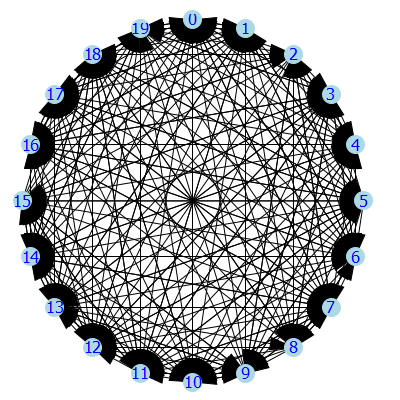
\includegraphics[width=.75\linewidth,height=.60\textheight,keepaspectratio]{graphs_img/graphs_18}\mbox{}\]

%%%%%%%%%%%%%%%%


\noindent
%%%%%%%%
%% INPUT:
\begin{minipage}[t]{4.000000em}\color{red}\bfseries
(\% i61)	
\end{minipage}
\begin{minipage}[t]{\textwidth}\color{blue}
is\_sconnected(H);
\end{minipage}
%%%% OUTPUT:
\[\displaystyle \tag{\% o61} 
true\mbox{}
\]
%%%%%%%%%%%%%%%%


\noindent
%%%%%%%%
%% INPUT:
\begin{minipage}[t]{4.000000em}\color{red}\bfseries
(\% i62)	
\end{minipage}
\begin{minipage}[t]{\textwidth}\color{blue}
vertex\_in\_degree(10,\ H);
\end{minipage}
%%%% OUTPUT:
\[\displaystyle \tag{\% o62} 
13\mbox{}
\]
%%%%%%%%%%%%%%%%


\noindent
%%%%%%%%
%% INPUT:
\begin{minipage}[t]{4.000000em}\color{red}\bfseries
(\% i63)	
\end{minipage}
\begin{minipage}[t]{\textwidth}\color{blue}
vertex\_out\_degree(10,\ H);
\end{minipage}
%%%% OUTPUT:
\[\displaystyle \tag{\% o63} 
7\mbox{}
\]
%%%%%%%%%%%%%%%%

\newpage
\section*{Заключение}
\addcontentsline{toc}{section}{Заключение}

\textbf{Цель исследования: } познакомиться с специализированным пакетом $graphs$, создать различные графы, изобразить их и исследовать их свойства. \\

\textbf{Использованные средства: }исследование проводилось с помощью\\ функций программы wxMaxima.\\

\textbf{Результат: } были созданы графы и орграфы: с помощью задания множеств вершин и ребер, матрицы смежности, уже созданного графа, специального вида, случайные графы и орграфы с заданным количеством вершин, в которых каждое ребро присутствовало с указанной вероятностью.

Были построены их изображения с опциями по умолчанию и заданными. Были найдены матрицы смежности некоторых графов.

Для графа $F$ было выяснено, что он связный, не является деревом, не двудольный, гамильтоновый и не планарный. Так же для него были составлены списки вершин, степеней вершин и ребер. Были найдены его средняя степень вершин, минимальная, максимальная. Для вершины с номером 10 была определена ее степень и составлен список вершин, смежных с ней. Были найдены диаметр, перефирия, радиус, центр графа и эксцентриситет вершины с 10 для графа $F$.

Для орграфа $H$ выяснили, что он сильно связный, нашли степень исхода и захода вершины с номером 10.
\end{document}
